

\begin{figure*}[p]
	\centering

	\begin{subfigure}[b]{0.7\textwidth}
		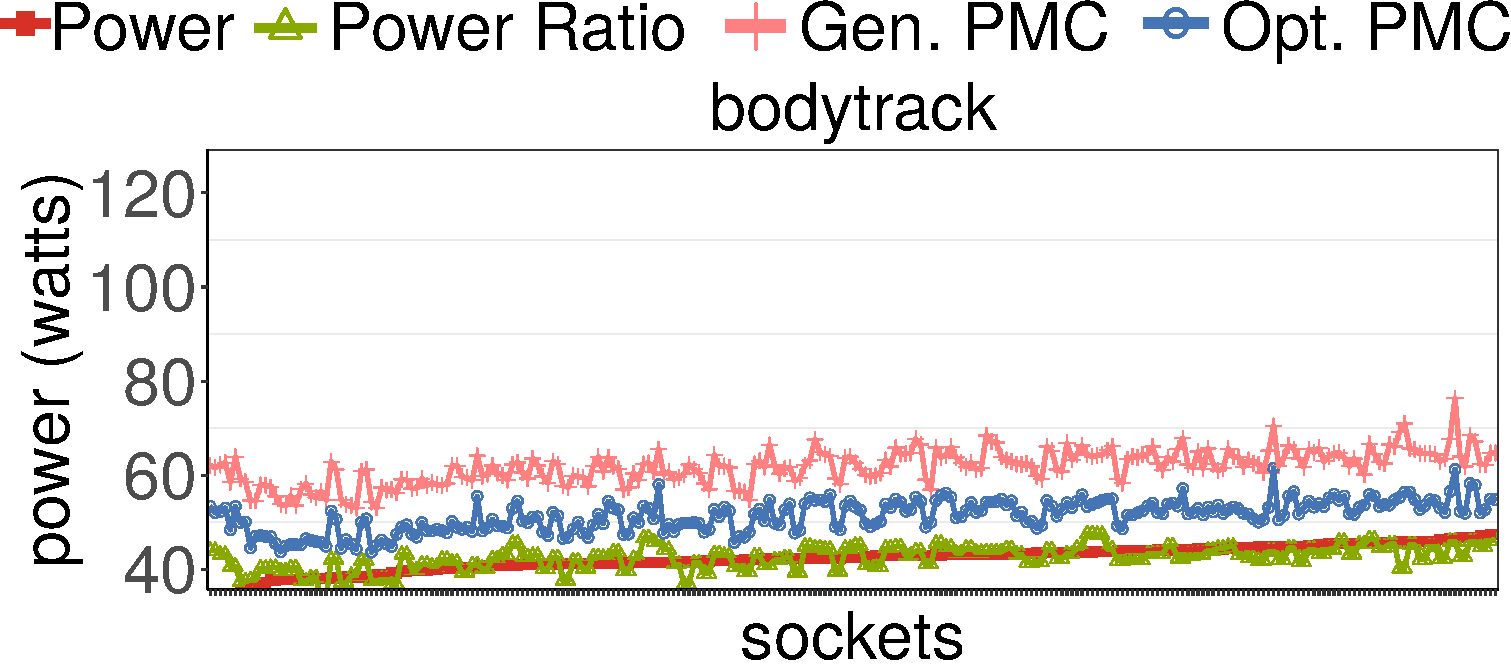
\includegraphics[width=\textwidth]{{power_aware_job_scheduling/figures/all_models_bodytrack_ncores12_pl115_power_eval}.pdf}
		\label{fig:bodytrack_trend}
	\end{subfigure}%

	\begin{subfigure}[b]{0.7\textwidth}
		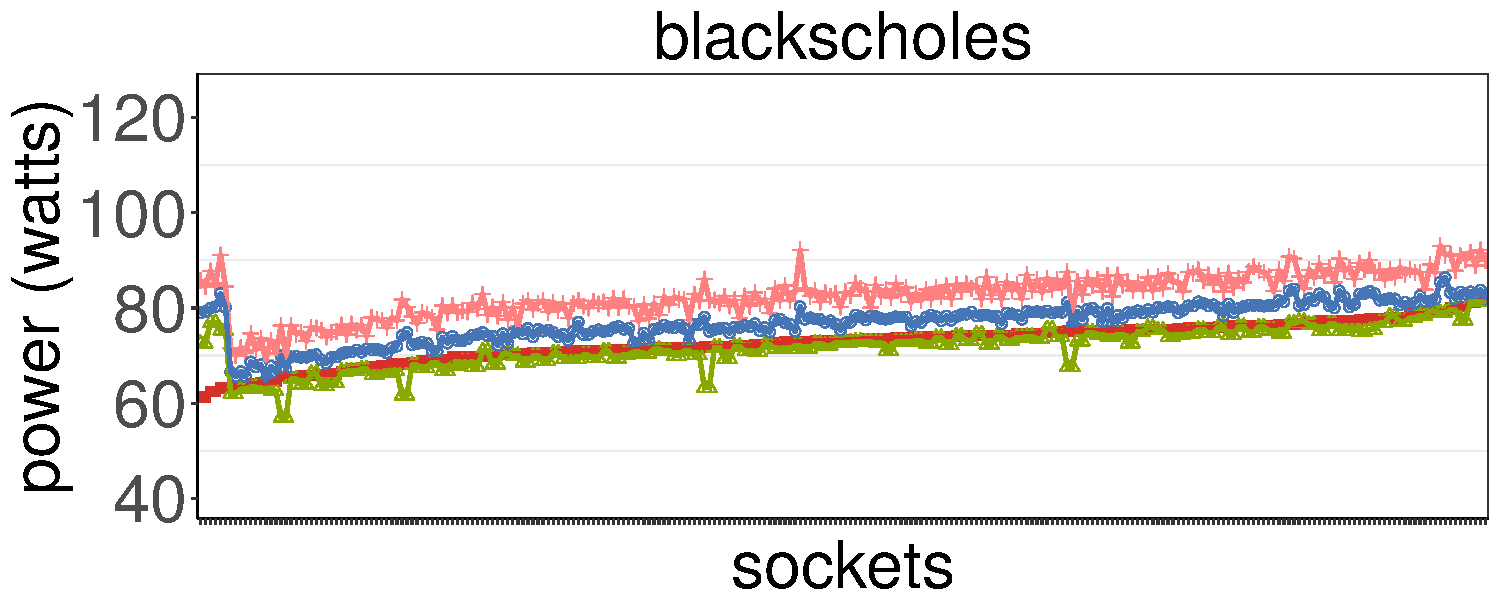
\includegraphics[width=\textwidth]{power_aware_job_scheduling/figures/all_models_blackscholes_ncores12_pl115_power_eval}
		\label{fig:blackscholes_trend}
  \end{subfigure}%

	\begin{subfigure}[b]{0.7\textwidth}
		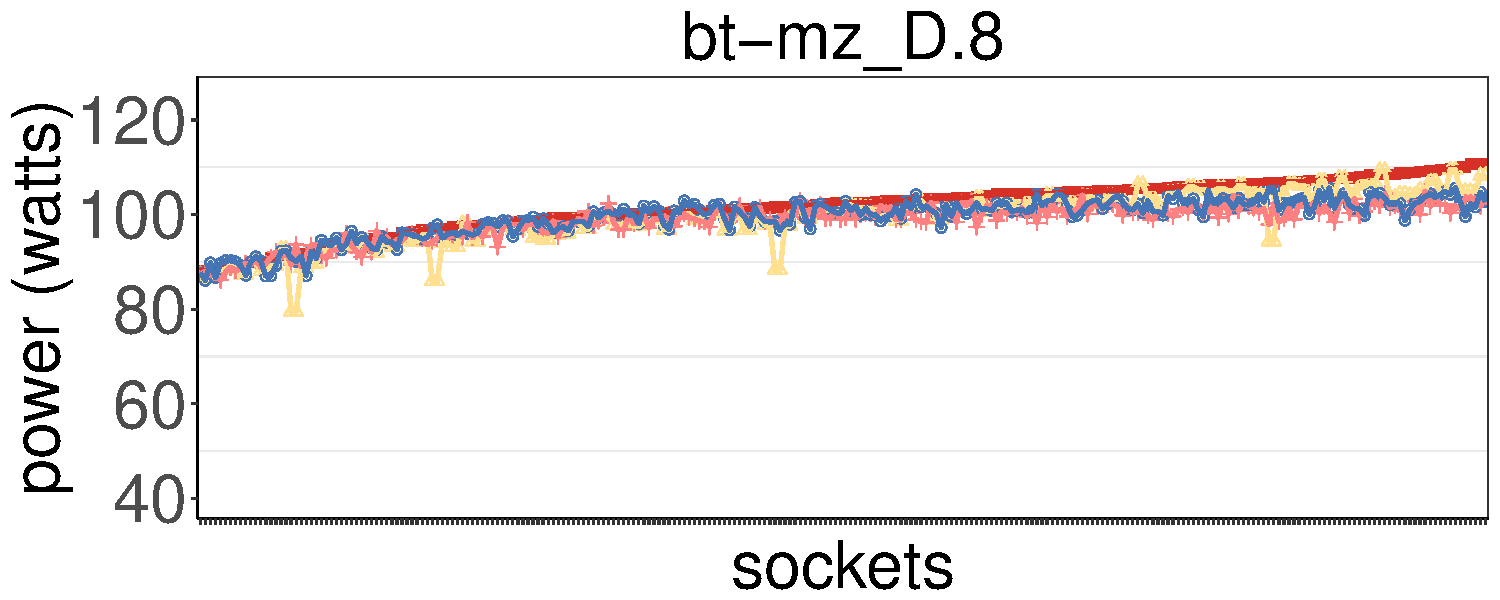
\includegraphics[width=\textwidth]{{power_aware_job_scheduling/figures/all_models_bt-mz_D.8_ncores12_pl115_power_eval}.pdf}
		\label{fig:bt-mz_D.8_trend}
	\end{subfigure}%

	\begin{subfigure}[b]{0.7\textwidth}
		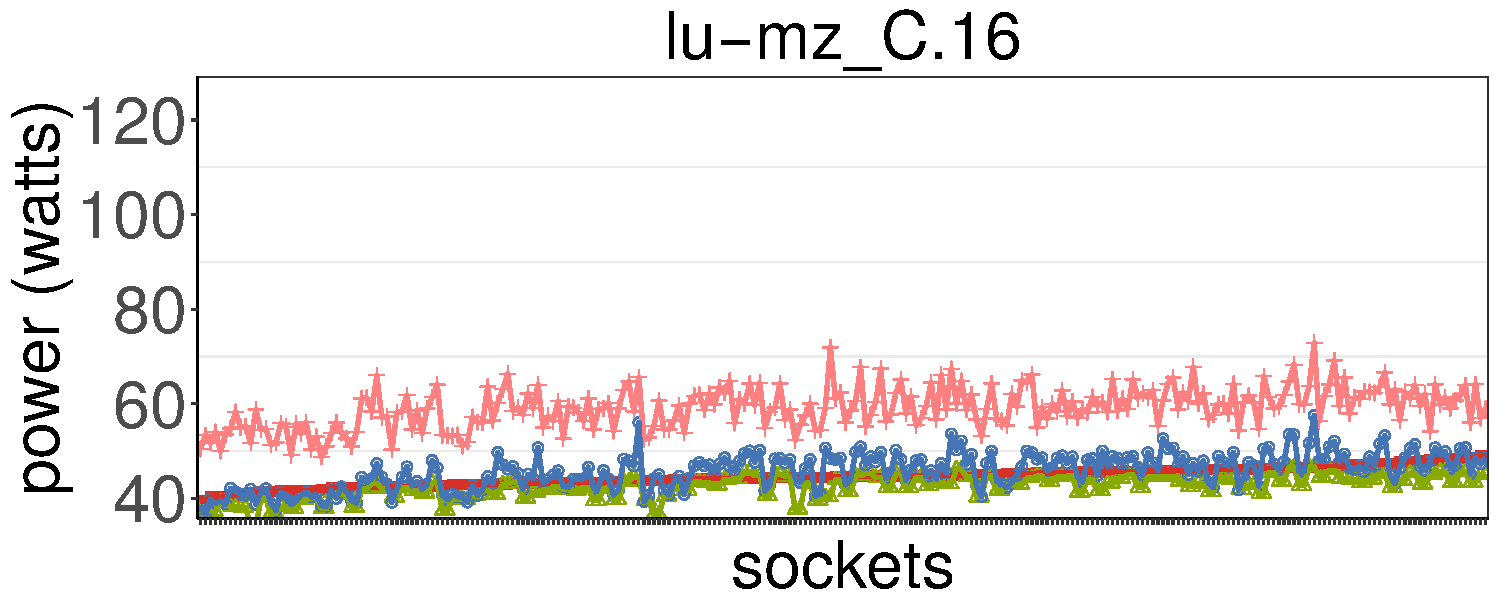
\includegraphics[width=\textwidth]{{power_aware_job_scheduling/figures/all_models_lu-mz_C.16_ncores12_pl115_power_eval}.pdf}
		\label{fig:lu-mz_D.16_trend}
	\end{subfigure}%
%		  \vspace{-0.5cm}
      \caption{Average power consumption and corresponding predictions across 256 sockets. Each point shows the average power consumption of an application for a specific socket.  Sockets are ordered on y axis 
							from most to least power efficient, according to their actual power consumption, while corresponding predictions are shown for each socket and prediction model. \textit{Power} refers to the actual power measured, while \textit{Gen. PMC} and \textit{Opt. PMC} are abbreviations for Generic and Optimized PMC models, respectively.}
			\label{fig:var_pred_trend}
%		  \vspace{-0.3cm}
%	\vspace{-.5cm}
\end{figure*}

\subsection{Model Validation}
\label{sec:model_validation}
In this section we experimentally validate the prediction models presented in Section~\ref{sec:variability_prediction}.  
We analyze the models in terms of Mean Absolute Percentage Error (MAPE) (see Equation \ref{eq:mape})  between predicted and real values.

Figure~\ref{fig:model_power_pred_error} shows the MAPE values of the average power predictions for all applications over all sockets.  
The error bars show the standard deviation of the MAPE metric, computed over all the 256 sockets.
These results correspond to the Power Ratio prediction model, presented 
in Section~\ref{sec:naive_model}, and the two variations of the PMC-based approach, which are both presented in Section~\ref{sec:pmcs_model}.
Optimized PMC performs well, achieving an average error below 10\%.
In most cases it is
matched by the Power Ratio model, which actually performs significantly better than Optimized PMC in the cases of \textit{bodytrack} and \textit{facesim}.
The Generic PMC model performs poorly, which is the reason why it is not used by any of our job scheduling policies.
The reason for its poor performance is the misleading contribution of some of the architectural components.
%All models perform well under most cases with an error value below 10\%. 

\begin{figure*}[ht!]
	\centering
% \hspace*{-1cm}
  \begin{subfigure}[b]{.9\textwidth}
    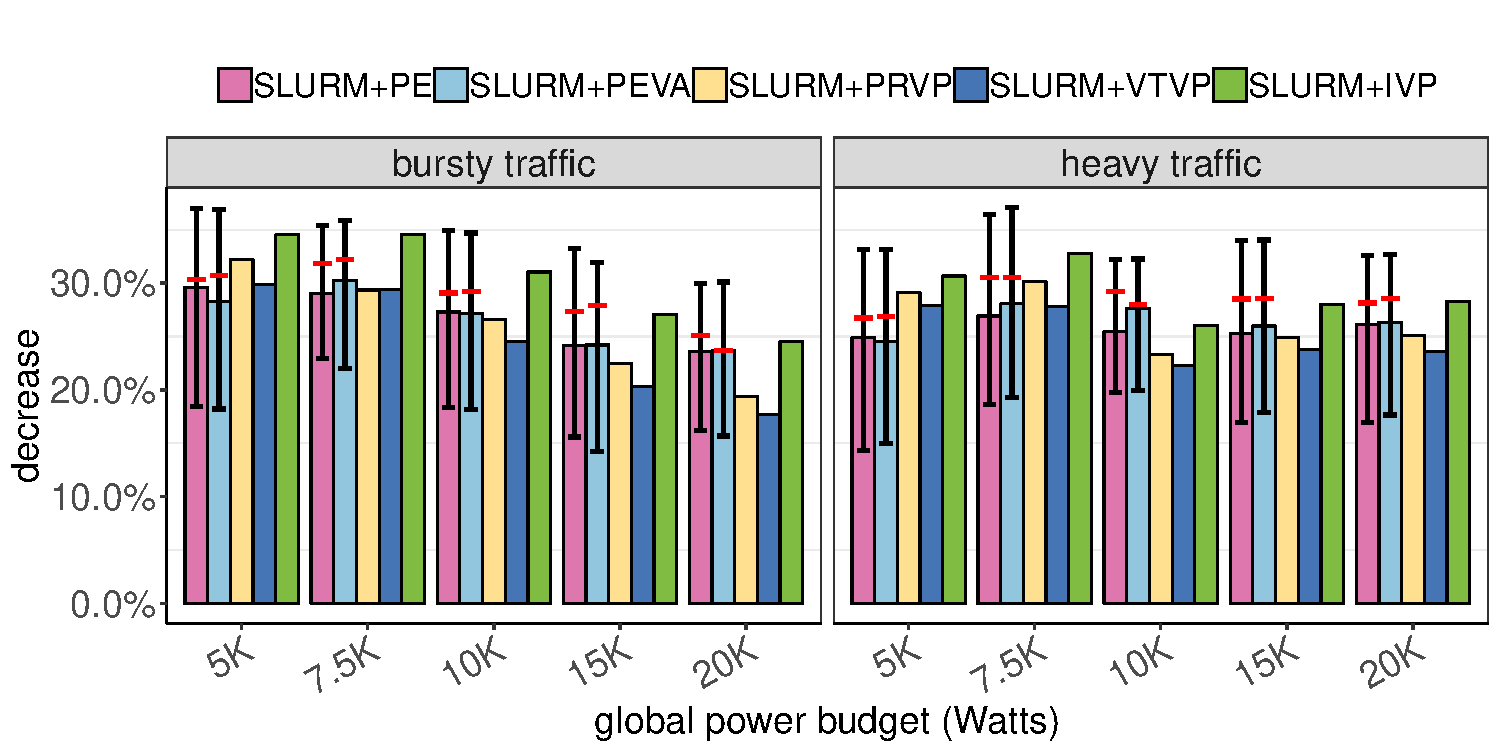
\includegraphics[width=\textwidth]{power_aware_job_scheduling/figures/average_turnaround_time_115W}
    \caption{Average turnaround time.}
    \label{fig:avg_turnaround_time_115W}
  \end{subfigure}%

	\begin{subfigure}[b]{.9\textwidth}
  	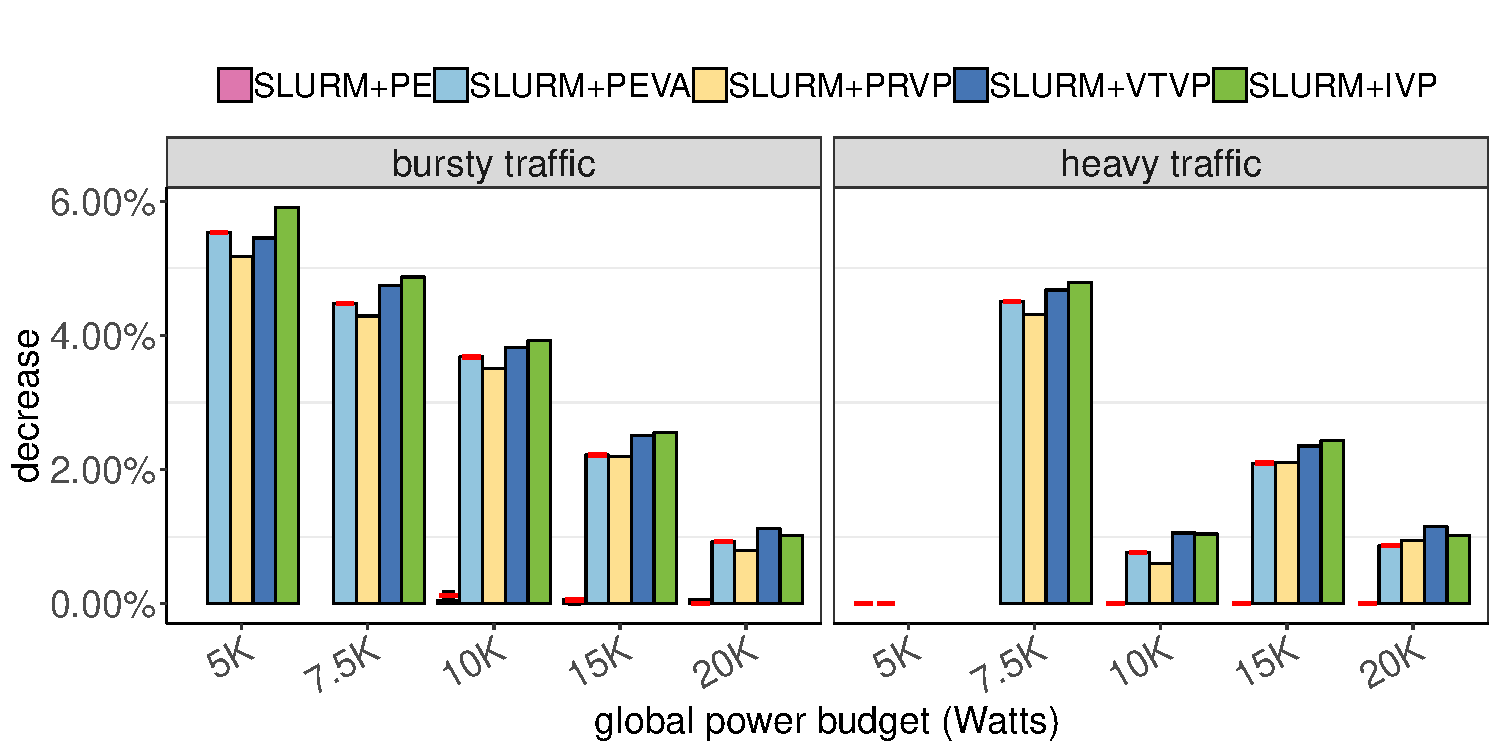
\includegraphics[width=\textwidth]{power_aware_job_scheduling/figures/total_energy_115W}
		\caption{Total energy consumption.}
    \label{fig:total_energy_115W}
  \end{subfigure}%

	\caption{	Impact of power-aware scheduling policies, under different power budgets and traffic scenarios, for job turnaround time and total energy consumption.
						Percentages represent improvement over the \DefaultSched~ policy.  For \PESched~ and \PEVASched~ policies the error bars represent the maximum and minimum benefit when we over and under estimate 
						power consumption, respectively.  We obtain these estimations according to the most and least power efficient sockets.  The red lines on the error bars, show the maximum benefit by 
						under estimating power consumption, without exceeding this budget.}
	\label{fig:policy_comparison}
	\vspace{.5cm}
\end{figure*}



Moreover, figure~\ref{fig:model_peak_pred_error} shows the prediction error and standard deviation when predicting the
peak power consumption reached per each application. 
Peak power predictions are crucial to the scheduling policies presented in Section~\ref{sec:job_sched_policies}, 
since they are fundamental to estimate the system-wide power consumption
and to keep it below the global power budget.  
As in the average prediction case, the Generic PMC model performs significantly worse than the Power Ratio and the Optimized PMC ones.
%Optimized PMC performs well again, but in most cases it is 
%matched by the Power Ratio model and it actually performs significantly better then Generic PMC in the cases of \textit{dedup} and \textit{facesim}.
%As observed in both power_aware_job_scheduling/figures, the Generic PMC model performs poorly, which is the reason why it is not used by any of our job scheduling policies.
%The reason for its poor performance is the misleading contribution of some of the architectural components.  To mitigate this problem  we can either use a larger set of applications 
%for training the model, or fine tune it to only consider the most relevant components for each applicPower Ratio.  We chose the latter approach, which is the Optimized PMC model. 

%Since we want to capture the power consumption variability, it is imperative to see the predictions for each socket individually.
Figure~\ref{fig:var_pred_trend} shows the average power consumption for all applications and the predicted average power 
consumption for Power Ratio, Generic and Optimized PMC models. Each point on the figure shows the power consumption (y axis) for a socket (x axis),
for the corresponding application. In the case of the multi-node MPI applications, a point shows the average power consumption among different process ranks of the same
application, relevant to that socket. 
Data is ordered on the x axis from least to most power consuming socket, according to the 
actual power consumption.  
Each point for the three prediction models shows the predicted power consumption for the corresponding socket, as ordered by
the actual power consumption.  
Overall prediction values follow the same trend as actual values, capturing power variability to a satisfactory degree.
\par
%There are two cases, \textit{bodytrack} and \textit{facesim}, where the prediction error is high.  
%However, the problem is not that our models do not capture the variability.
%Instead, they miss-predict power consumption to the same extend for all the sockets.
%If we observe Figure~\ref{fig:var_pred_trend} we can see how these two problematic cases both exhibit lower power consumption compared to the rest of the
%applications.  
%Although \textit{dedup} also consumes less than 60 Watts, it uses only one core for the largest portion of its execution, while \textit{bodytrack} and
%\textit{facesim} use 12 and 8 respectively, which is not
%This behavior is not 
%captured by our training set.
%, which leads to these prediction errors.   

Our results show that all three models are able to predict the power consumption variability in most cases.  However, it is possible to
miss-predict if an application's behavior is not well represented by the benchmarks used for training.  
In our evaluation there are two
such cases, \textit{bodytrack} and \textit{facesim}, that although they are effectively using more than 8 cores, their power consumption remains below 60 Watts.  
The Generic PMC model
 shows the least tolerance to these cases, with errors as high as 45\%, which is not acceptable.  
The Optimized PMC model, however,
which is a fine tuned version of the Generic one, mitigates the issue by selecting the most relevant architectural components for prediction. 
%Moreover, the Optimized PMC model has a smaller standard error deviation in most cases than the Power Ratio technique, which indicates that it predicts power more accurately.

\subsection{Variability-Aware Scheduling Evaluation}
\label{sec:job_sched_eval}
In this Section we evaluate the two novel scheduling policies, \PRVSSched~ and \PMCVSSched~, which are presented in Section~\ref{sec:job_sched_policies}.
We compare them to four other scheduling policies, \DefaultSched~, \PESched~, \PEVASched~ and \IVSSched~, which are also described in~\ref{sec:job_sched_policies}.
\DefaultSched~ policy implements SLURM's logic in our simulator, with the addition of power-awareness and power backfilling.
\PESched~ and \PEVASched~ employ state-of-the-art features of power-aware policies ~\cite{patki:2013:eho:2464996.2465009,7515666,Gholkar:2016:PTH:2967938.2967961},
while \IVSSched~ demonstrates and ideal scenario, where prediction is 100\% accurate.  
The evaluation is done based on a simulator, as described in Section~\ref{sec:simulator}, by feeding it performance and power traces from actual executions on the catalyst cluster.
For our experiments we generate random job workloads composed of nine applications from the PARSECSs suite and seven multi-node jobs from NAS-MZ, simulating both bursty and heavy traffic scenarios
(see Section~\ref{sec:cluster_traffic}).
%This workload consists of 2524 jobs in total. 
The main objective of each policy is to improve the cluster's performance and energy consumption, while keeping the total energy consumption below a certain global power budget. 
All policies treat power as a limited resource 
and depending on a predicted or estimated power peak for each job, they restrict the number of running jobs to only those that can be accommodated by the given global power budget.  
%As described above, policies use different prediction models or estimations based on power profiling.

Figure~\ref{fig:policy_comparison} compares the different policies in terms of average job turnaround time reduction and total energy reduction. 
Results consider four different system-wide power budgets, 5K, 7.5K, 10K, 15K and 20K Watts and two traffic scenarios (x axis).  
Our workloads require 25K Watts to run using the whole cluster without any power restrictions.  In the 5KW case, the \DefaultSched~ is forced to drop jobs
that use 64 sockets, since it estimates that these jobs require more power than available to the system.  The 7.5KW budget, is the minimum budget that allows 
\DefaultSched~ to run jobs that demand 64 socket.  
The benefit shown in percentages on y axis is over the \DefaultSched~ policy, for the corresponding power budget and traffic.

\begin{figure*}[p]
        \centering
  \begin{subfigure}[b]{.9\textwidth}
    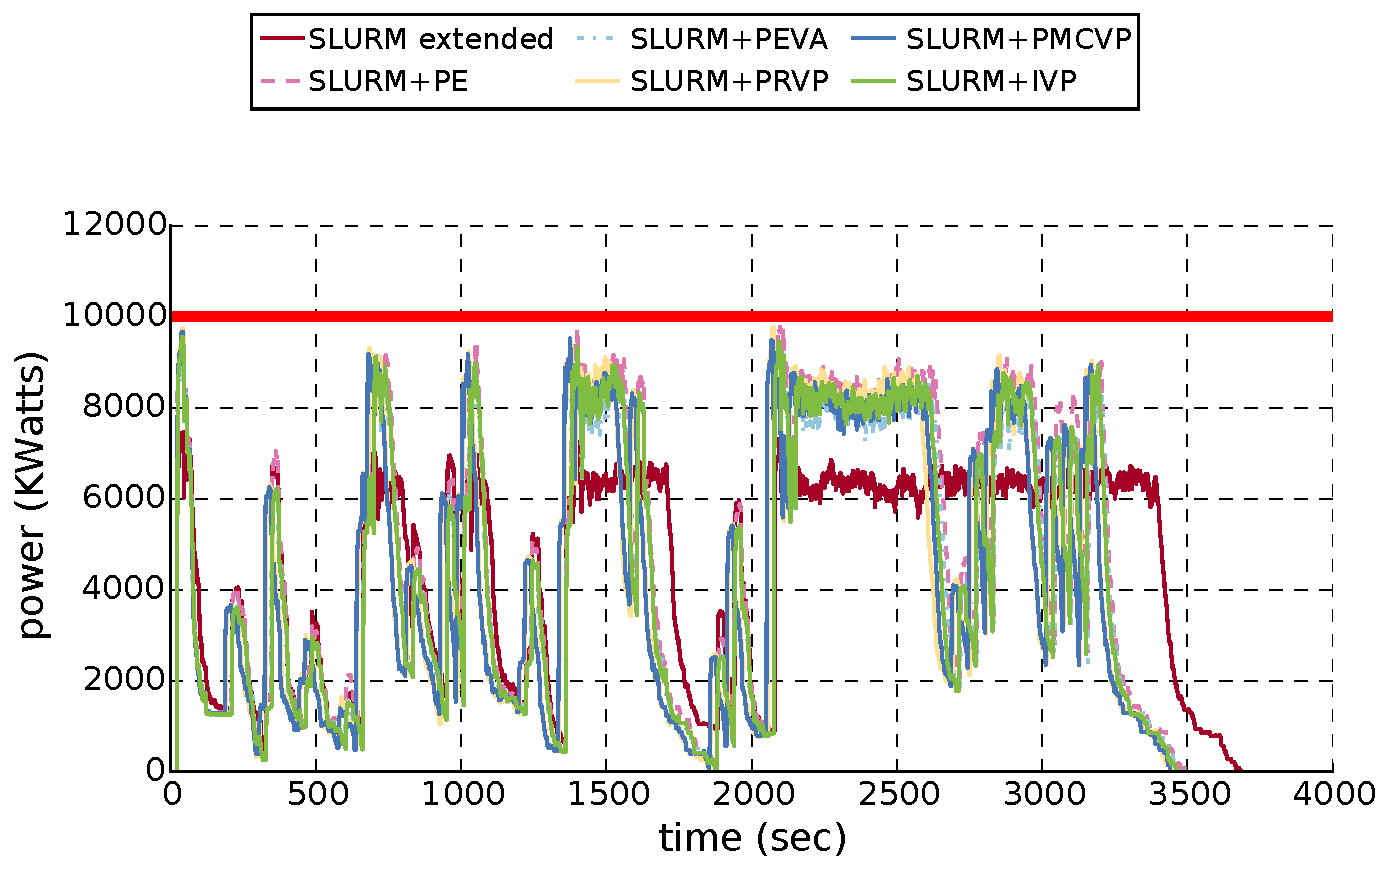
\includegraphics[width=\textwidth]{power_aware_job_scheduling/figures/net_power_trace_default}
    \caption{System's net power trace over all sockets on the cluster when power profiling is performed on a socket with medium power consumption.}
    \label{fig:net_power_trace}
  \end{subfigure}%

	\begin{subfigure}[b]{.9\textwidth}
   	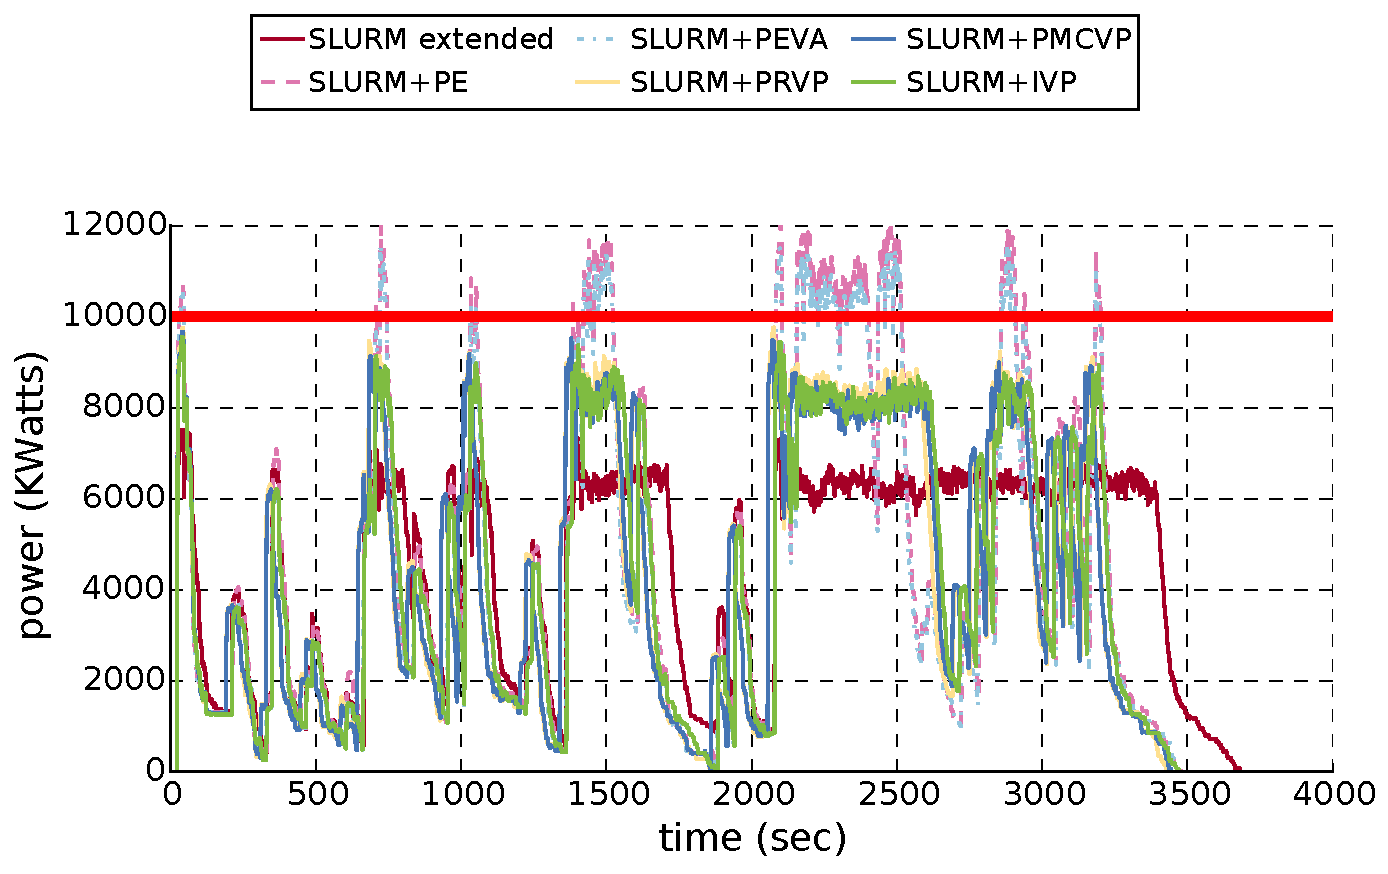
\includegraphics[width=\textwidth]{power_aware_job_scheduling/figures/net_power_trace_under_estimate}
    \caption{System's net power trace over all sockets on the cluster when power profiling is performed on a socket with low power consumption.}
  	\label{fig:net_power_trace_under_estimation}
  \end{subfigure}%

  \caption{Power traces of net power consumption over all sockets, for bursty traffic scenario. Line at 10KWatts shows the system-wide power budget.  Figure on the left shows that estimation-based policies, 
								\PESched~ and \PEVASched, fails to respect the global power budget, when underestimating an applications power consumption.  Contrary, \PRVSSched~ and \PMCVSSched, 
								which rely on our prediction model, have more precise estimations of the jobs' real consumption and always maintain the net power consumption below the budget.}
        \label{fig:net_power_trace_under_estimate}
       \vspace{.5cm}
\end{figure*}



Unlike our proposed policies, which use prediction models to compute the power 
consumption of each job on each socket, the power-estimation-based plocies, \PESched~ and \PEVASched, use a single power estimation obtained from power profiling on a single socket.  
Due to the power variability of each socket, it is possible that the estimation varies according to the variability of the socket used for profiling.
This variance impacts the policies' efficiency. 
The error bars show the range of improvement achieved by the \PESched~ and \PEVASched~ policies.  
Maximum and minimum values correspond to the performance obtained 
when using power profiles from the most and least efficient sockets respectively.     
Underestimating power by using a power efficient socket allows more sockets to get allocated, but the net power consumption of the system can exceed the system-wide power budget, as we show in Figure~\ref{fig:net_power_trace_under_estimate} and discuss in Section~\ref{sec:budget}. 
The red line on the error bars, show the maximum benefit achieved by under-estimating power consumption, without exceeding the 
system-wide power budget.

The average job turnaround time reduction of \PESched, \PEVASched, \PRVSSched~ and \PMCVSSched~ over \DefaultSched~ policy is shown in Figure~\ref{fig:avg_turnaround_time_115W}. 
For both traffic scenarios, we observe that the benefit of the  \PESched, \PEVASched, policies reaches an average benefit of \AvgJTT\%, matching the \IVSSched~ policy.  
The \PESched~ and \PEVASched~ policies also perform equally well, when estimation is based on an average socket (average in terms of power efficiency).
The benefit range from \EstMaxJTT\% to \EstMinJTT\%.
Considering power variability during scheduling decisions does not seem to play a major role here, since the variability-agnostic \PESched~ match the performance of the \PEVASched~ and even 
the \PRVSSched~ and \PMCVSSched~ policies.  However, the accuracy of the estimation or prediction is important for improving turnaround time.  The less accurate  \PESched~ and \PEVASched~ policies achieve lower benefits in the more power restricted scenarios.

Figure~\ref{fig:total_energy_115W} shows the reduction in the system-wide energy consumption.  
Both traffic scenarios' benefits increase as the system wide power budget is reduced.
When less power is available, considering variability is important for energy saving, since we can choose to always use the most power efficient sockets.  
Note that under heavy traffic, the 5K scenario offers no benefit.  This is because a significant number of multi-node jobs are dropped by the \DefaultSched~ since they appear to require more 
power than available to the system.  As a result, \DefaultSched~ runs a lighter workload than he rest of the policies.  This also happens in the bursty scenario, but since the workload only contains
a few 64 socket jobs that are dropped, we still observe significant benefits. 
%This is also the reason why 
%we observe less energy savings for 15K and 20K power budgets under heavy traffic, when compared to the bursty traffic scenario.  Under heavy traffic and 20K we are always using all the sockets,
%even the less power efficient one, but as less power becomes available to the system, the scheduler is forced to reduce the number of concurrent sockets and is now able to only use the more power 
%efficient ones.
\PESched, which is variability-agnostic, offers no benefit over the \DefaultSched~ policy.  \PEVASched, which prioritizes allocation of power efficient sockets, 
matches the energy savings of the \PRVSSched~ and \PMCVSSched~ policies.
Overall, accounting for power variability can have a significant impact on energy efficiency reaching \MaxEnergy\% on the most energy-restricted scenarios.


\subsection{Meeting the System Power Budget}
\label{sec:budget}
Power profiling is a necessary step in order to get a power consumption estimation and not fall back to conservative power budgeting, as done in the \DefaultSched~ policy.  
In contrast to the \PRVSSched~ and \PMCVSSched~ policies proposed by this thesis, the \PESched~ and \PEVASched ones are subject to the variability of the socket when power profiling a job.  
Results in Figure~\ref{fig:policy_comparison} show how the benefits of \PESched~ and \PEVASched~ policies vary, depending on estimation precision.  
Over-estimating
power consumption causes more conservative scheduling decisions, resulting in smaller benefits.  
Under-estimating appears to improve results, but this is misleading.
It allows the schedulers to allocate more sockets, but under a false premise. 
Figure~\ref{fig:net_power_trace} shows the system-wide power consumption of all policies over time under bursty traffic,
when power profiling is performed on a socket with medium power consumption. 
The horizontal line at 10KW on the y axis shows the system-wide power budget and all policies remain below it.
In contrast, Figure~\ref{fig:net_power_trace_under_estimation} shows the system-wide power consumption for the same traffic, when power profiling is done on a power-efficient socket.  
In this scenario we can observe that
\PESched~ and \PEVASched~ policies (dashed lines) exceed the power budget for 16.3\% of the execution time.

Results shown across Section~\ref{sec:job_sched_eval} prove that our proposed \PRVSSched~ and \PMCVSSched~ policies can improve energy efficiency up to \MaxEnergy\% (\AvgEnergy\% on average) over 
simple solutions commonly used. 
Moreover, job turnaround time is reduced up to \MaxJTT\% (\AvgJTT\% on average).
Compared to the \PEVASched~ policy, which is variability-aware, our method is more robust  
as none of the  \PESched~ and \PEVASched~ policies
can guarantee that the system-wide power budgets are respected. 
%while their performance directly depends on the precision of the estimation provided.  
%Contrarily, our \PRVSSched~ and \PMCVSSched~ policies can mitigate socket variability when estimating a jobs power consumption.  
